\documentclass{mrl}
\usepackage[utf8]{inputenc}
\usepackage[T2A]{fontenc}
\usepackage[english, russian]{babel}
\usepackage{amsthm,amsmath}
\usepackage{listings}
\lstset{basicstyle=\ttfamily\footnotesize,breaklines=true}
\usepackage{hyperref}
\usepackage{graphicx}
\usepackage{enumerate}
\renewcommand{\figurename}{Рисунок}
\renewcommand{\tablename}{Таблица}

\title{Техническая записка по цепной реакции в процессе отслеживания в рамках протокола CryptoNote 2.0}
\authors{Шурэ Ноезер (Surae Noether)\footnote{\texttt{surae.noether@protonmail.com}}, Саранг Ноезер (Sarang Noether)\footnote{\texttt{sarang.noether@protonmail.com}} и Адам Маккензи (Adam Mackenzie)\footnote{\texttt{lab@getmonero.org}}}
\affiliations{Исследовательская лаборатория Monero (Monero Research Lab)}
\date{12 сентября 2014 }

\type{ИССЛЕДОВАТЕЛЬСКИЙ БЮЛЛЕТЕНЬ}
\ident{MRL-0001}

\begin{document}

\begin{center}
{\bfАннотация}
\end{center}

В этом исследовательском бюллетене описана вероятная атака на системы анонимности на базе кольцевых подписей. В качестве основы нами был взят криптовалютный протокол CryptoNote 2.0, который был предположительно опубликован Николасом Ван Саберхагеном в 2012 г. Ранее было продемонстрировано, что функция обеспечения неотслеживаемости, скрывающая пару одноразовых ключей, может зависеть от неотслеживаемости всех ключей, используемых для составления кольцевой подписи. Это создаёт возможность цепных реакций в процессе отслеживания между кольцевыми подписями, что приводит к критической потере свойства неотслеживаемости во всей сети, если параметры были выбраны не надлежащим образом, и если человек, проводящий атаку, контролирует достаточную часть сети. Тем не менее подписи по-прежнему остаются одноразовыми, и любая такая атака, вполне вероятно, может ослабить ту защиту сети от анализа, которую обеспечивает протокол CryptoNote. Данный исследовательский бюллетень прошёл независимую экспертизу и отражает только результаты внутренних исследований.

\section{Вступление}
У протокола CryptoNote есть одна проблема: моя анонимность зависит от вашей анонимности. Если я использую $5, 6$ или $18$ ваших выходов при составлении своей кольцевой подписи, то \emph{вы} можете вычислить реальный выход подписи. Если вы тратите все $5, 6$ или $18$ выходов, не прибегая к помощи сторонних выходов в качестве миксинов, в своей кольцевой подписи, вы раскрываете сами себя как отправителя средств, и уже любой наблюдатель сможет увидеть истинного подписанта моей транзакции. Это может не иметь никакого значения, если вы тратите ваши выходы открыто в законных коммерческих или других целях. Таким образом, любая из сторон, владеющая значительной частью UTXO, может отследить чужие транзакции и в любой момент выложить информацию в сеть. Кто-то может счесть эту проблему абстрактной, криптовалютным вариантом реализации закона Грешема, согласно которому плохие деньги со временем вытесняют хорошие. Если набор непотраченных выходов транзакции (UTXO) будет связан со множеством транзакций, которые не являются анонимными, то круг способов обеспечения неотслеживаемости кольцевых подписей сузится. Здесь \emph{необходимо} отметить, что даже при таком сценарии пары одноразовых ключей (так называемые «скрытые адреса»), используемые протоколом CryptoNote, не нарушаются, а следовательно, и анонимности пользователей ничто не угрожает. Скорее, данная атака нарушает механизм обеспечения неотслеживаемости \emph{между} одноразовыми кольцевыми подписями, но и это развитие событий некоторым образом беспокоит. Следовательно, даже если добросовестные пользователи могут случайно провести эту атаку, злоумышленники тем более могут наводнить сеть собственными наборами UTXO и сделать остальных отслеживаемыми.

Намерение проводящего атаку, вероятно, может состоять в реализации стратегии «накачки и сброса» с целью подрыва репутации криптовалюты, а возможно, в слежении за другими пользователями или же в нежелании нести дополнительные расходы при добавлении сторонних непотраченных выходов транзакций в свои кольцевые подписи. Во всех случаях, несмотря на имеющуюся \emph{априори} надежду, любой отдельно взятый пользователь всегда в принципе должен быть заинтересован в использовании большого количества миксинов в своих кольцевых подписях как из соображений личной безопасности, так и в общих интересах. Но на практике нам этого ожидать не приходится. Может случиться некая версия так называемой трагедии общих ресурсов, и из-за небольшой группы пользователей появится возможность отследить в сети всех и каждого.

Тем не менее нам следует думать о лесе в целом, а не о деревьях, так как любой пользователь всегда может создать тривиальную кольцевую подпись без каких-либо дополнительных выходов, просто выставив свои выходы в линию на обозрение, и тут мы сталкиваемся с проблемой второго порядка. Была раскрыта новая транзакция, подвергая риску раскрытия любые кольцевые подписи, которые использовались в новой раскрытой транзакции в качестве «маскировочных» миксинов. Возможно ли возникновение цепной реакции, \emph{даже если злоумышленник прекратит активно проводить атаки на раннем этапе истории монеты}? Настоящий исследовательский бюллетень был написан с целью анализа этой проблемы, определения вероятности наличия консервативного пути проведения такой атаки, а также оценки сетевых параметров, которые гарантируют постепенное снижение уровня неотслеживаемости.

\section{Настройка пассивной атаки}
Каждый, у кого в колледже были курсы по теории вероятности, сталкивался с такой задачей, даже если не знал, как она решается:

\begin{quote}
В урне есть $N$ шариков двух цветов. У нас есть $N_B$ шариков чёрного цвета и $N_W$ шариков белого цвета, при этом $N_B + N_W = N$ имеет фиксированное значение. Мы достаём $M$ шариков из урны. Какова вероятность, что все шарики, которые мы вынули из урны окажутся чёрными? И какова вероятность, что все шарики, которые мы вынули из урны окажутся белыми? Если $0 \leq m \leq M$, какова вероятность, что у нас будет $m$ чёрных шариков и $M-m$ белых шариков?
\end{quote}

Когда мы формулируем проблему таким образом, мы сразу же переходим к гипергеометрическому распределению. Функция масс вероятности \[\frac{\binom{N_B}{B}\binom{N - N_B}{M - B}}{\binom{N}{M}}\] может использоваться для вычисления вероятности, что все шарики в моей руке чёрные (при заданном $B=M$), и мы можем использовать удобную формулу, которую можно найти в любом бесплатном онлайн учебнике или в Википедии, или где бы то ни было, чтобы вычислить вероятность любого отдельно взятого события. Это один из лучших вариантов распределения.

Мы сыграем в следующую игру: если все шарики, которые были вынуты мной, окажутся чёрными, я брошу новый чёрный шарик в урну, когда буду брать очередную пригоршню. В противном случае, когда я буду брать новые шарики, я брошу туда белый шарик. Точно так же, как это происходит с шариками, всё обстоит и с монетами на базе протокола CryptoNote: можно рассматривать каждый шарик в качестве атомной единицы (CryptoNote аналог «сатоши»), отслеживаемого в наборе UTXO сети CryptoNote. Цвет указывает на то, кто владеет шариком: чёрный цвет означает, что шариком владеет злоумышленник, а белый - наоборот.

Допустим, Лиза хочет перевести некоторое количество денег в Milhouse (которые положат шарик в свою сумку). Набор UTXO, который Лиза возьмёт, чтобы создать свои кольцевые подписи, будет содержать $N$ выходов транзакции, из которых $N_B$ выходов будет контролироваться Бёрнсом (чёрные шарики, если допустить, что остальные белые). Формула, приведённая выше, идеально нам подходит. Лиза составила свою подпись, включив в неё $M \leq N$ миксинов\footnote{Мы называем {\it миксином} сторонний выход, включаемый в транзакцию.} (она взяла пригоршню шариков, чтобы решить, шарик какого цвета добавить в урну), и что если все они контролируются Бёрнсом? Ну, тогда, \emph{если} Бёрнс потратит свои выходы без миксинов\footnote{Что (и это необходимо снова подчеркнуть) может быть совершенно невинным актом, а вовсе не атакой!}, транзакция Лизы также будет раскрыта. Более того, помимо транзакции Лизы, \emph{вообще любая} кольцевая подпись, в которой будут использоваться только подписи Бёрнса, теперь фактически может рассматриваться как часть контролируемого Бёрнсом набора (с точки зрения неотслеживаемости), даже если Бёрнс не контролирует приватные ключи. Следует отметить, что при таком сценарии цепная реакция обязательно произойдёт: Бёрнс раскрывает не только собственные выходы транзакции, но также, в свою очередь, раскрывает выход Лизы. В данном случае нами было сделано четыре допуска:

\begin{enumerate}[(i)]
\item Бёрнс контролирует начальную пропорцию каким-либо образом ставшего известным ему набора UTXO;
\item При создании всех новых транзакций их кольцевые подписи генерируются на основе текущего набора UTXO единообразным беспорядочным образом без замены;
\item Все новые транзакции используют один и тот же обязательный минимальный уровень содержания миксинов (размер пригоршни $M$);
\item Бёрнс получает контроль над транзакциями в том и только в том случае, если их кольцевые подписи состоят исключительно из контролируемых Бёрнсом транзакций (то есть Бёрнс прекращает добавлять транзакции в систему в течение временного периода $t=0$).
\end{enumerate}

Мы можем изменить наши допуски, чтобы усилить или ослабить атаку согласно нашему сценарию. Например, атака будет слабее, если в некоторых транзакциях будет использоваться более обязательного минимума миксинов. И атака станет сильнее, если Бёрнсу также удастся получить контроль над транзакциями, самостоятельно генерируя их, то есть он будет действовать не пассивно. Тем не менее кажется разумным при некоем среднем варианте развития сценария интерпретировать всё следующим образом: Бёрнс изначально контролирует часть набора UTXO до того, как будут созданы «флуд»-транзакции или честные транзакции. Итак, что же произойдёт? Защита сети от масштабного снижения уровня неотслеживаемости при таком сценарии является просто делом умного технического решения. Если же мы сможем защитить сеть от масштабной деградации при более негативных сценариях, тем лучше, но начнём с другого. Назовём это «рождественской» атакой, поскольку наша модель подобна неожиданному всплеску экономической деятельности до того, как настоящий злоумышленник сможет отреагировать (из-за простоты кодирования), а также потому, что атака может быть проведена совершенно невинным пользователем, просто и не анонимно отправляющим свои деньги на вполне законных основаниях.

Так как гипергеометрическое распределение работает довольно хорошо, что мы можем ожидать от этой игры? Ну, давайте проанализируем результаты по \emph{одной отдельно взятой транзакции}. Допустим, $M$ является минимальным количеством миксинов дс наля всей сети. Какова вероятность, что все подписи с миксинами $M$ будут контролироваться Бёрнсом? Если такая возможность велика, то довольно вероятно, что новые транзакции также будут «контролироваться» Бёрнсом, даже если ему приходится раскрывать выходы транзакций, которые он контролирует. К слову, чем больше транзакций CryptoNote контролируется одной недобросовестной стороной, тем слабее становится свойство \emph{неотслеживаемости} новых транзакций. Рассмотрим следующий числовой пример.

Предположим, что в нашем анонимном наборе есть $N=10^3$ выходов транзакций (не считая реального выхода, принадлежащего Лизе) и что Бёрнс контролирует $pN$ этих транзакций для некоторого $0 \leq p \leq 1$. Обозначим как $\Pr(p)$ вероятность, что любая из этих кольцевых подписей (использующих три миксина) подписана исключительно выходами, принадлежащими Бёрнсу. Эта вероятность описывает, грубо говоря, что новый шарик Лизы будет чёрным или белым. В таблице \ref{3mixins} приводятся примеры значений $\Pr(p)$ для этого случая.

\begin{table}[!h]
\begin{center}
\begin{tabular}{c|c|c}
$p$ & $pN$ & $\Pr(p)$ \\ \hline
$10^{-3}$ & $1$ & $0$ \\
$10^{-2}$ & $10$ & $7.22\times 10^{-7}$ \\
$10^{-1}$ & $100$ & $9.73 \times 10^{-4}$\\
$0.5$ & $500$ & $0.125$
\end{tabular}
\caption{Если Бёрнс контролирует $pN$ выходов транзакций из анонимного набора $N=10^3$ выходов, мы демонстрируем вероятность $\Pr(p)$ что, с точки зрения Бёрнса, выход Лизы можно отследить, если допустить, что Лиза использует три миксина в своей кольцевой подписи. Иначе говоря, в начале масштабного моделирования, если Бёрнс контролирует половину всех транзакций, мы можем ожидать, что он будет «видеть» примерно $12.5\%$ всех новых транзакций.}
\label{3mixins}
\end{center}
\end{table}

Как мы интерпретируем данную таблицу? Если Бёрнс контролирует только один выход из анонимного набора, невозможно, чтобы все три выхода в кольцевой подписи принадлежали ему. Если Бёрнс контролирует десять выходов, то вероятность того, что кольцевая подпись Лизы реально контролируется Бёрнсом, составляет всего $0.00000722$. Это так незначительно, что в среднем понадобится примерно $13.8$ миллиона подписей из этого анонимного набора, чтобы увидеть какие-то совпадения. Если Бёрнс контролирует $100$ выходов, то вероятность того, что подпись, сгенерированная Лизой, контролируется Бёрнсом, составляет $0.000973$, то есть мы можем начать поиск совпадений уже среди примерно $100,000$ подписей. Наконец, если Бёрнс контролирует половину всех выходов, то $12.5\%$ всех новых транзакций будут иметь подписи, состоящие полностью из его выходов, и Бёрнс будет получать $1$ из каждых $8$ новых транзакций, и доля Бёрнса в наборе UTXO сократится со временем, если он ничего не предпримет.

В таблице \ref{2mixins} нами представлены те же значения, что и в таблице \ref{3mixins} , но с условием наличия двух миксинов. В этом случае, если Бёрнс контролирует половину выходов, в последствии каждый из четырёх новых выходов будет реально контролироваться Бёрнсом. Если Бёрнс контролирует $10\%$ выходов, только $1$ из $1000$ новых транзакций будет контролироваться им. Очевидно, что это не так хорошо, как в случае с $3$ миксинами, но всё же и не так страшно; даже если Бёрнс контролирует половину всех транзакций, вероятность того, что новая кольцевая подпись будет принадлежать ему, составляет всего $25\%$. Следовательно, его доля в наборе UTXO также сократится со временем, если он ничего не предпримет.

\begin{table}[!h]
\begin{center}
\begin{tabular}{c|c|c}
$p$ & $pN$ & $\Pr(p)$ \\ \hline
$10^{-3}$ & $1$ & $0$ \\
$10^{-2}$ & $10$ & $9.01\times 10^{-5}$ \\
$10^{-1}$ & $100$ & $9.91 \times 10^{-3}$\\
$0.5$ & $500$ & $0.25$ \\
\end{tabular}
\end{center}
\caption{Если Бёрнс контролирует $pN$ выходов транзакций из анонимного набора $N=10^3$ выходов, мы демонстрируем вероятность $\Pr(p)$, что новый выход будет раскрыт при проведении атаки, если допустить, что Лиза использует два миксина в своей кольцевой подписи. Иначе говоря, в начале масштабного моделирования, если Бёрнс контролирует все транзакции, мы можем ожидать, что он «захватит» примерно $25\%$ всех новых транзакций.}

\label{2mixins}
\end{table}

\section{Методы Монте-Карло и результаты}

Приготовьтесь к тому, что сейчас вам придётся столкнуться с рядом обозначений. Мы берём параметры $N_{B_0}, N_{W_0}$ и $M$, где $N_{B_0}$ обозначает начальное количество чёрных шариков, имеющихся у Бёрнса, $N_{W_0}$ обозначает начальное количество белых шариков, а $M$ является минимальным количеством миксинов. Мы станем играть итеративно. Сначала мы записываем изначальную пропорцию непотраченных транзакций, которыми владеет Бёрнс, как $P_0 = N_{B_0}/(N_{B_0} + N_{W_0})$В очередной $i^{ой}$ итерации мы добавляем $N_i = (N_{B_0} + N_{W_0} + i)$ шарик в сумку. Мы берём случайное количество $u$ из $(0,1)$ и сравниваем его с гипергеометрической функцией масс, как описано выше. Если $u \leq \binom{N_{B_i}}{M}/\binom{N_i}{M}$, то следующий шарик будет чёрным, поэтому мы итеративно повторяем $N_{B_i} = N_{B_{i-1}}+1$. Независимо от выбора $u$, мы итеративно повторяем $N_{i+1} = N_{i} + 1$, и если нам необходимо вычислить $N_W$ мы можем просто вычесть. После некоторого количества итераций, скажем, $I$ итераций, обычно это достаточное количество итераций, чтобы удвоить или учетверить набор UTXO, мы останавливаем игру и смотрим на пропорцию чёрных шариков, $P_F = N_{B_I}/N_I$. Тем не менее, так как нас интересует только то, \emph{сколько новых шариков являются чёрными} (а не сколько всего чёрных шариков), нашим показателем успешности атаки Бёрнса станет значение $\widehat{P}_F = (N_{B_I} - N_{B_0})/I$, количество чёрных шариков, полученных Бёрнсом во время игры, поделённое на количество шариков, добавленных в сумку.

Вышеописанный процесс является единой моделью. Для каждого набора параметров $(N_{B_0}, N_{W_0}, M)$ мы получаем результат $\widehat{P}_F$, который определяется как результат последовательности случайных экспериментов и является случайной переменной. Таким образом, мы проводим $37$ испытаний и в результате экспериментов получаем выборочное среднее и выборочную дисперсию. Изначально нами наблюдались доверительные интервалы в $95\%$, но они настолько незначительны, что в конечном счёте их можно просто игнорировать. Нами моделируется набор UTXO, начинающийся с $5000$ транзакций и заканчивающийся $20000$ транзакций. Следовательно, мы берём $(20000P_F - 5000P_I)/15000$, то есть пропорцию \emph{предположительно честных транзакций, захватываемых Бёрнсом.} На рисунке \ref{fig1} приводятся результаты нашего моделирования для $N_B+N_W = 5000$ и $M=1, 2, 3$ и $4$ (обязательное минимальное количество миксинов), в случае, если набор UTXO учетверяется с добавлением честных транзакций (то есть $15,000$ новых транзакций необходимы новые кольцевые подписи). Горизонтальная ось показывает начальную пропорцию набора UTXO, контролируемую Бёрнсом, которая варьируется от $0.0$ до $1.0$, а вертикальная ось показывает окончательную пропорцию \emph{новых} транзакций в наборе UTXO, контролируемом Бёрнсом, которая также варьируется от $0.0$ до $1.0$. Следует отметить, что \emph{любое число выше нуля на оси $y$ указывает на снижение уровня безопасности}.

\begin{figure}[!h]
\centering
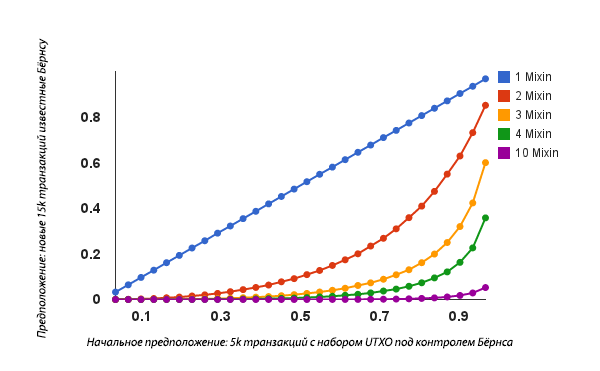
\includegraphics[width=0.95\textwidth,height=0.95\textheight,keepaspectratio]{burns.png}
\caption{На этом рисунке показана (просим прощения за бледность цвета) «успешность атаки» Бёрнса. Мы можем увидеть, что при повышении количества миксинов успешность снижается на всём графике. Чтобы объяснить всё читателю, который, возможно, начал сразу с этого графика, в данном случае реализуется следующий сценарий: злой парень Бёрнс, имея начальную часть (ось-$x$) набора UTXO, состоящего из $5000$ выходов транзакций. Затем в сеть попадает $15,000$ новых транзакций, от Лизы к Милхаусу, от Гомера к Мардж и так далее, в результате чего набор UTXO увеличивается в четыре раза. После этого Бёрнс может потратить свою часть $P_I$ набора UTXO без каких-либо миксинов и, как следствие, нарушит неотслеживаемость части из $15,000$ предположительно честных транзакций. Нами показана эта часть $\widehat{P}_F$ как функция $P_I$. В случае с $10$ миксинами при таких параметрах. Бёрнсу понадобится $55\%$ набора UTXO, чтобы охватить любое событие учетверения и $87\%$ UTXO, чтобы захватить всего $1\%$ события учетверения.}
\label{fig1}
\end{figure}

Очевидно, что $\widehat{P}_F$ однообразно повышается как функция $P_0 = N_B/(N_B + N_W)$, но ситуация улучшается по мере увеличения количества кольцевых подписей. Следует отметить, что нашим данным присущи некоторые динамические системные проблемы. Если вы сравниваете графики $P_F$ и $P_I$, (а не наш $\widehat{P}_F$ и $P_I$) то это можно интерпретировать как функцию развития динамической системы с дискретным временем, необходимую, чтобы увидеть, как доля Бёрнса со временем уменьшится до нуля при количестве миксинов большем либо равном $\geq 2$. Мы можем ожидать, что при сценарии с $1$ миксином количество в урне будет стохастически скакать вверх и вниз по линии $y=x$ без заметного, как ожидается, движения в каком-либо направлении случайным образом. Тем не мене, так как нам необходимо $M \geq 2$ миксинов, любая цепная реакция, скажем так, прекратится сама по себе. Доля Бёрнса в наборе UTXO уменьшится до нуля со временем, если не будет предпринято каких-либо действий. Результаты нашего моделирования показывают, что любое обязательное количество миксинов $\geq 2$ позволит системе довольно быстро восстановиться после пассивной атаки. Код, использованный нами для генерирования данных, вероятно, можно улучшить. Тем не менее вы сможете найти его на \texttt{http://goo.gl/dGj5TZ}, а для создания рисунков мы воспользовались Google Documents.

\section{Критическая масса, медленные цепные реакции, активные атаки: прочие вопросы}

Вспомним, что нами был поставлен вопрос: «Возможна ли критическая цепная реакция?» А также связанный с первым второй вопрос: «Какие сетевые параметры следует выбрать, чтобы возможная цепная реакция прекратилась сама по себе?» Таким образом, что нам нужно для создания критической массы? Рассмотрим снова задачу с урной. Что происходит с содержимым урны, после того как мы начинаем игру, по мере того как мы забрасываем чёрные или белые шарики в урну по мере развития игры? Помните, чёрные шарики — это те, которые будут раскрыты; если мы вынем все чёрные шарики, это будет означать, что следующий шарик, который мы добавим в урну, будет чёрным. При сценарии с критической массой в урне должно быть достаточное количество шариков, после чего Бёрнс станет брать всё больше и больше этих чёрных шариков. Даже если $P_F > P_I$, мы можем ожидать появления некоторой критической массы, но этого не происходит. Исключение составляют случаи числовой границы, $P_F \leq P_I$. В случае с $2$ и большим количеством миксинов наша цепная реакция сойдёт на нет очень быстро.

Цепные реакции замедляются всё быстрее по мере роста количества миксинов. Таким образом, использование одного миксина является неприемлемым в случае с любой валютой, поскольку анонимный недобросовестный пользователь может «наводнить» сеть контролируемыми им транзакциями в надежде, что они в конечном счёте позволят ему контролировать большую часть набора UTXO. В значительной степени \emph{в дальнейшем} это сделает все транзакции отслеживаемыми (по крайней мере, с точки зрения Бёрнса), и Бёрнсу не придётся делать ничего после того, как его первые транзакции попадут в набор UTXO. Это \emph{фиксированная начальная стоимость} для проводящего атаку, а результатом является нескончаемый поток информации в форме отслеживаемых транзакций других пользователей, что, очевидно, является экономической катастрофой. Это так важно, что мы выделим курсивом: \emph{любая монета на базе протокола CryptoNote, использующая только $1$ миксин, уязвима с точки зрения медленной цепной реакции, в результате которой владелец всего нескольких приватных ключей сможет нейтрализовать механизм обеспечения неотслеживаемости других пользователей}. Требование к использованию по крайней мере $2$ миксинов спасёт те транзакции, которые добровольно проводятся вообще без использования миксинов, и, вероятно, снизит масштаб цепной реакции. На самом деле подойдёт любое количество более $1$ Этого будет достаточно для того, чтобы цепная реакция прекратилась сама по себе и не распространилась на всю сеть, и чем больше миксинов будет использоваться, тем лучше. Безусловно, обусловленное протоколом, используемое во всей сети обязательное минимальное количество миксинов $M=10$ предположительно вызовет «раздувание» блокчейна, что может препятствовать признанию монеты, но это также обеспечит определённую безопасность с точки зрения размера сети. Следовательно, должно быть определено некоторое оптимальное обязательное минимальное количество миксинов. Мы не более чем предлагаем использовать $M=2$ в качестве обязательного минимума на основе протокола и советуем пользователям использовать столько миксинов, сколько пожелают их маленькие сердца.

Следует отметить, что наш сценарий может быть несколько иным, если мы изменим параметры нашей модели или наши допуски и включим в него злоумышленников, проводящих активные атаки. Давайте по-быстрому рассмотрим параметры. Мы можем рассматривать добавление каждого нового шарика как некое подталкивание Бёрнса к \emph{пассивному} владению. Если только Бёрнс не завладеет почти всеми входящими транзакциями, его доля в наборе UTXO со временем сойдёт на нет. Как наши параметры могут изменить этот процесс? Вспомним наши параметры:
\begin{enumerate}
\item $N_{B_0} = $ количество начальных атомных единиц, контролируемых Бёрнсом в наборе UTXO;
\item $N_{W_0} = $ количество оставшихся атомных единиц в наборе UTXO;
\item $M = $ обязательное минимальное количество миксинов, предусмотренное сетевым протоколом.
\end{enumerate}
Тем не менее нам действительно интересны $P_I = N_{B_0}/(N_{B_0} + N_{W_0})$ и $N_0 = N_{B_0} + N_{W_0}$. Выше мы увидели, как $P_I$ и $M$ в целом меняют результаты эксперимента. По мере роста значения N0 доля Бёрнса в наборе будет снижаться. Это означает, что даже если Бёрнс завладеет всеми входящими транзакциями, результаты для него будут хуже с точки зрения общей части набора UTXO, которой он будет владеть. Мы можем рассматривать размер набора UTXO в качестве массы. По мере её роста будет всё сложнее изменить её состояние.

Другим «скрытым» параметром в данном случае является то, «сколько новых транзакций добавляется». Мы спрятали это «под ковёр», просто сказав: «OK, размер набора UTXO увеличится в четыре раза в сравнении с начальным». Это несколько сократило пространство нашего параметра, и тем самым мы также снизили важность $N_0$ как параметра. На самом деле нам известно, как изменяется $N$, поэтому мы легко можем определить изменение любой статистики, $T(N)$, относительно «изменения величины популяции» и называем это чувствительностью:
\[S = \frac{T(N_f) - T(N_o)}{N_f - N_o} = \frac{T(4\cdot N_o) - T(N_o)}{3N_o}\]
которая, если близка к нулю, не предполагает каких-либо отношений, а если сильно отличается от нуля, предполагает сильное отношение (положительное или отрицательное). Мы можем легко вычислить изменение логарифма статистики относительно логарифма популяции и назвать это чувствительностью:
\[S = \frac{\log(T(N_f)) - \log(T(N_0))}{\log(N_f)-\log(N_o)} = \frac{1}{4}\log\left(\frac{T(4\cdot N_o)}{T(N_o)}\right)\]
в этой версии мы даже не наблюдаем $N_f$ как части формулы, а просто мультипликативный множитель $N_f/N_o = 4$. Тем не менее мы считаем, что не имеет смысла представлять анализ полномасштабного пространства параметров этой модели.

Теперь давайте поговорим об изменении допусков. Одним из очевидных хитрых изменений, которые можно было бы реализовать в рамках данной модели, является изменение допуска (iv). Чтобы смоделировать более агрессивную атаку, чем «рождественское» случайное раскрытие, мы бы могли сделать такой вероятностный допуск:
\begin{enumerate}[(v)]
\item Бёрнс получает контроль над новыми транзакциями в результате последовательности испытаний по схеме Бернулли. Имея фиксированную вероятность $q$, Бёрнс генерирует транзакцию, которая, как ему известно, будет его, и с вероятностью $1-q$ появляется сторонняя транзакция и генерирует новую кольцевую подпись, которая может состоять исключительно из контролируемых Бёрнсом транзакций (то есть Бёрнс по-прежнему участвует в схеме).
\end{enumerate}
или же мы могли бы реализовать динамическую модель, в рамках которой злоумышленник Бёрнс попытался бы поддерживать минимальную часть набора UTXO, передавая свои транзакции в сеть всякий раз, когда его часть становилась меньше, секретно заданного им самим процента:
\begin{enumerate}[(v)]
\item Бёрнс получает контроль над новыми транзакциями в результате последовательности не автономных испытаний, подобных испытаниям по схеме Бернулли. С вероятностью $q(B,N)$, которая зависит как от количества UTXO, контролируемых Бёрнсом, $B$, так и общим набором UTXO, $N$, Бёрнс генерирует транзакцию, которая, как ему известно, будет его, и с вероятностью $1-q(B,N)$ появляется сторонняя транзакция и генерирует новую кольцевую подпись, которая может состоять исключительно из контролируемых Бёрнсом транзакций.
\end{enumerate}
Любая функция $q(B,N)$, которую Бёрнс попытается приблизить к $1$, когда отношение $B/N$ будет меньше предпочитаемого Бёрнсом, позволит ему увеличить свою долю в наборе UTXO. Безусловно, самой простой стратегией для Бёрнса будет просто заполнить сеть своими транзакциями как можно быстрее. Но, учитывая комиссии, это будет отнюдь не бесплатно.

Мы поднимаем вопрос параметров и допусков, поскольку работа по этой проблеме ещё не закончена. Мы узнали то, что нам как сетевым инженерам необходимо для того, чтобы элегантно снизить вероятность цепной реакции — необходимо использовать большое количество миксинов. Тем не менее на поверхность ещё не были подняты реально интересные вопросы. Один из нас решил эту проблему, пользуясь теорией графов, а другой — теорией вероятности. Следует отметить, что с течением времени UTXO с более высокой вероятностью будет выбран в качестве миксина, но столь же вероятно он может быть выбран из предыдущих транзакций пользователей, которые вообще не используют миксинов, что усложняет разумный выбор UTXO для создания кольцевой подписи путём равномерного распределения. Технически в случае с любым видом проблемы, связанной с «критической массой», существует проблема стабильного состояния, скрытая под поверхностью, и у нас есть некоторые соображения\footnote{Видели, что я сделал в этом плане?}, связанные с динамическими системами, которые позволят решить эту проблему. Может какой-нибудь студент захочет начать с того, на чём мы закончили, и внести свой вклад в дело криптовалютного сообщества, расширив исследования по теме.

\end{document}
